% --------------------------------------------------------------
% This is all preamble stuff that you don't have to worry about.
% Head down to where it says "Start here"
% --------------------------------------------------------------

\documentclass[12pt]{article}

\usepackage[margin=1in]{geometry}
\usepackage{amsmath,amsthm,amssymb}
\usepackage{graphicx}
\usepackage{subcaption}
\usepackage{algorithmicx}
\usepackage{algorithm}
\usepackage{algpseudocode}
\usepackage[colorlinks,linkcolor=blue]{hyperref}
\usepackage[noabbrev]{cleveref}
\usepackage{courier}
\usepackage{listings}
\usepackage{float}


\oddsidemargin 0in
\evensidemargin 0in
\textwidth 6.5in
\topmargin -0.5in
\textheight 9.0in

\newcommand{\ignore}[1]{}
\def\pp{\par\noindent}

\newcommand{\assignment}[4]{
\thispagestyle{plain}
\newpage
\setcounter{page}{1}
\noindent
\begin{center}
\framebox{ \vbox{ \hbox to 6.28in
{CIS 419/519: Applied Machine Learning \hfill #1}
\vspace{4mm}
\hbox to 6.28in
{\hspace{2.5in}\large\bf\mbox{Homework #2}}
\vspace{4mm}
\hbox to 6.28in
{{\it Handed Out: #3 \hfill Due: #4}}
}}
\end{center}
}

\makeatletter
\renewcommand{\fnum@algorithm}{\fname@algorithm}
\makeatother

\lstset{basicstyle=\footnotesize\ttfamily,breaklines=true}
\lstset{framextopmargin=50pt,frame=bottomline}


\begin{document}

\assignment{Fall 2024}{0}{August 28}{7:59 pm September 4}

% --------------------------------------------------------------
%                         Start here
% --------------------------------------------------------------


{\bf Name: }  Alan Liu Wu\\

{\bf PennKey:} alanlwu\\

{\bf PennID:} 41855518

\section{Declaration}
\begin{itemize}
\item \textbf{Person(s) discussed with:} \textit{None}
\item \textbf{Affiliation to the course: student, TA, prof etc.} \textit{None}
\item \textbf{Which question(s) in coding / written HW did you discuss?} \textbf{\textit{None}}
\item \textbf{Briefly explain what was discussed.} \textit{None}
\end{itemize}

\section{Multiple Choice \& Written Questions}

\begin{enumerate}
\item %Question 1 
\begin{enumerate}
\item \textbf{C}
\item \textbf{A}
\end{enumerate}

\item
\begin{enumerate}
\item \textbf{D}
\item \textbf{A}
\end{enumerate}

\item
  \begin{enumerate}
  \item \textbf{A}
  \item \textbf{A}
  \end{enumerate}

\item
  \begin{enumerate}
  \item \textbf{B}
  \item We are given that 
  \begin{align}
    Var(x) = E[(X-E[X])^{2}] \\ 
    = E[(x^{2} - 2xE[x] + E[x]^{2})] \\ 
    = E[x^2] - E(2xE[x]) + E[E[x]^2] \\ 
    = E[x^2] - 2 \cdot E[x] \cdot E[x] + E[x]^2 \\
    = E[x^2] - 2E[x]^2 + E[x]^2 \\ 
    = E[x^2] - E[x]^2
  \end{align}
  We know that $E[2xE[x]] = 2E[x]E[x] = 2E[x]^2$ because $E[x]$ is a constant. Furthermore
  we know that $E[E[x]^2] = E[x]^2$ because $E[x]$ is a constant. Thus, our equation for variance 
  $Var(x) = E[(X-E[X]^2)]$ reduces down to $E[x^2] - E[x]^2$.
  \end{enumerate}
 \item
 \begin{enumerate}
     \item \textbf{C}
     \item \textbf{D}
     \item \textbf{A}
 \end{enumerate}
\item 
 \begin{enumerate}
    
    \item 
      We are given a 2x2 matrix. We can find the eigenvalues of a 2x2 matrix by solving the following equation: 
      $det(A- \lambda \cdot I) = 0$. Since A is 2x2 we know then $I = \begin{bmatrix} 1 & 0 \\ 0 & 1 \end{bmatrix}$. And also, 
      because A is a 2x2 matrix, then the determinant of any 2x2 matrix given elements $ \begin{bmatrix} a & b \\ c & d \end{bmatrix}$ 
      $det(M) = ad-bc$. Thus, we can solve for the eigenvalues of A by solving the equation: \\ 
      \begin{align}
        det(A - \lambda \cdot I) = 0 \notag \\ 
       = det(\begin{bmatrix} 4-\lambda & 2 \\ 1 & 5-\lambda \end{bmatrix}) = 0 \notag \\
        = (4-\lambda)(5-\lambda) - 2 = 0 \notag \\ 
        = 20 - 9 \lambda + \lambda^{2} - 2 = 0 \notag \\ 
        = \lambda^2 - 9\lambda + 18 = 0 \notag \\ 
        = (\lambda - 6)(\lambda - 3) = 0 \notag \\ 
        \lambda = 6, 3 \notag
      \end{align}
     Thus, the two eigenvalues for the matrix A are 6 and 3. 
    \item  \textbf{C}
 \end{enumerate}
\end{enumerate}

\section{Python Programming Questions}

% Complete questions in your iPython notebook and place all results here.
  \begin{figure}[H]
      \centering
      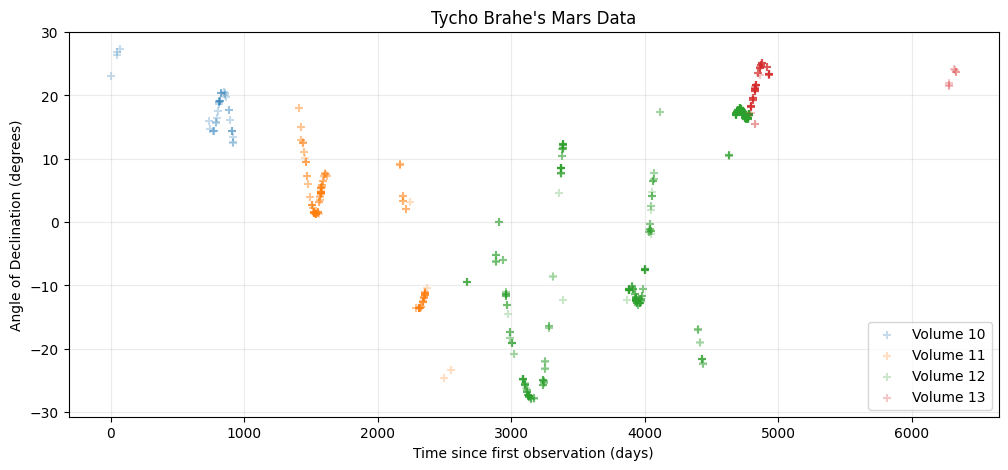
\includegraphics[width=\textwidth]{fig1.png}
      \caption{Figure 1}
      \label{fig:fig1}
  \end{figure}

\end{document} 